\documentclass[twoside]{book}

% Packages required by doxygen
\usepackage{fixltx2e}
\usepackage{calc}
\usepackage{doxygen}
\usepackage[export]{adjustbox} % also loads graphicx
\usepackage{graphicx}
\usepackage[utf8]{inputenc}
\usepackage{makeidx}
\usepackage{multicol}
\usepackage{multirow}
\PassOptionsToPackage{warn}{textcomp}
\usepackage{textcomp}
\usepackage[nointegrals]{wasysym}
\usepackage[table]{xcolor}

% NLS support packages
\usepackage[T2A]{fontenc}
\usepackage[russian]{babel}

% Font selection
\usepackage[T1]{fontenc}
\usepackage[scaled=.90]{helvet}
\usepackage{courier}
\usepackage{amssymb}
\usepackage{sectsty}
\renewcommand{\familydefault}{\sfdefault}
\allsectionsfont{%
  \fontseries{bc}\selectfont%
  \color{darkgray}%
}
\renewcommand{\DoxyLabelFont}{%
  \fontseries{bc}\selectfont%
  \color{darkgray}%
}
\newcommand{\+}{\discretionary{\mbox{\scriptsize$\hookleftarrow$}}{}{}}

% Page & text layout
\usepackage{geometry}
\geometry{%
  a4paper,%
  top=2.5cm,%
  bottom=2.5cm,%
  left=2.5cm,%
  right=2.5cm%
}
\tolerance=750
\hfuzz=15pt
\hbadness=750
\setlength{\emergencystretch}{15pt}
\setlength{\parindent}{0cm}
\setlength{\parskip}{3ex plus 2ex minus 2ex}
\makeatletter
\renewcommand{\paragraph}{%
  \@startsection{paragraph}{4}{0ex}{-1.0ex}{1.0ex}{%
    \normalfont\normalsize\bfseries\SS@parafont%
  }%
}
\renewcommand{\subparagraph}{%
  \@startsection{subparagraph}{5}{0ex}{-1.0ex}{1.0ex}{%
    \normalfont\normalsize\bfseries\SS@subparafont%
  }%
}
\makeatother

% Headers & footers
\usepackage{fancyhdr}
\pagestyle{fancyplain}
\fancyhead[LE]{\fancyplain{}{\bfseries\thepage}}
\fancyhead[CE]{\fancyplain{}{}}
\fancyhead[RE]{\fancyplain{}{\bfseries\leftmark}}
\fancyhead[LO]{\fancyplain{}{\bfseries\rightmark}}
\fancyhead[CO]{\fancyplain{}{}}
\fancyhead[RO]{\fancyplain{}{\bfseries\thepage}}
\fancyfoot[LE]{\fancyplain{}{}}
\fancyfoot[CE]{\fancyplain{}{}}
\fancyfoot[RE]{\fancyplain{}{\bfseries\scriptsize Создано системой Doxygen }}
\fancyfoot[LO]{\fancyplain{}{\bfseries\scriptsize Создано системой Doxygen }}
\fancyfoot[CO]{\fancyplain{}{}}
\fancyfoot[RO]{\fancyplain{}{}}
\renewcommand{\footrulewidth}{0.4pt}
\renewcommand{\chaptermark}[1]{%
  \markboth{#1}{}%
}
\renewcommand{\sectionmark}[1]{%
  \markright{\thesection\ #1}%
}

% Indices & bibliography
\usepackage{natbib}
\usepackage[titles]{tocloft}
\setcounter{tocdepth}{3}
\setcounter{secnumdepth}{5}
\makeindex

% Hyperlinks (required, but should be loaded last)
\usepackage{ifpdf}
\ifpdf
  \usepackage[pdftex,pagebackref=true]{hyperref}
\else
  \usepackage[ps2pdf,pagebackref=true]{hyperref}
\fi
\hypersetup{%
  colorlinks=true,%
  linkcolor=blue,%
  citecolor=blue,%
  unicode%
}

% Custom commands
\newcommand{\clearemptydoublepage}{%
  \newpage{\pagestyle{empty}\cleardoublepage}%
}

\usepackage{caption}
\captionsetup{labelsep=space,justification=centering,font={bf},singlelinecheck=off,skip=4pt,position=top}

%===== C O N T E N T S =====

\begin{document}

% Titlepage & ToC
\hypersetup{pageanchor=false,
             bookmarksnumbered=true,
             pdfencoding=unicode
            }
\pagenumbering{alph}
\begin{titlepage}
\vspace*{7cm}
\begin{center}%
{\Large P\+R\+OF site \\[1ex]\large 0.\+4 }\\
\vspace*{1cm}
{\large Создано системой Doxygen 1.8.13}\\
\end{center}
\end{titlepage}
\clearemptydoublepage
\pagenumbering{roman}
\tableofcontents
\clearemptydoublepage
\pagenumbering{arabic}
\hypersetup{pageanchor=true}

%--- Begin generated contents ---
\chapter{Иерархический список классов}
\section{Иерархия классов}
Иерархия классов.\begin{DoxyCompactList}
\item \contentsline{section}{Main}{\pageref{class_main}}{}
\item mysqli\begin{DoxyCompactList}
\item \contentsline{section}{DB}{\pageref{class_d_b}}{}
\end{DoxyCompactList}
\item \contentsline{section}{User}{\pageref{class_user}}{}
\end{DoxyCompactList}

\chapter{Алфавитный указатель структур данных}
\section{Структуры данных}
Структуры данных с их кратким описанием.\begin{DoxyCompactList}
\item\contentsline{section}{\hyperlink{class_d_b}{DB} }{\pageref{class_d_b}}{}
\item\contentsline{section}{\hyperlink{class_main}{Main} }{\pageref{class_main}}{}
\item\contentsline{section}{\hyperlink{class_user}{User} }{\pageref{class_user}}{}
\end{DoxyCompactList}

\chapter{Структуры данных}
\hypertarget{class_d_b}{}\section{Класс DB}
\label{class_d_b}\index{DB@{DB}}
Граф наследования\+:DB\+:\begin{figure}[H]
\begin{center}
\leavevmode
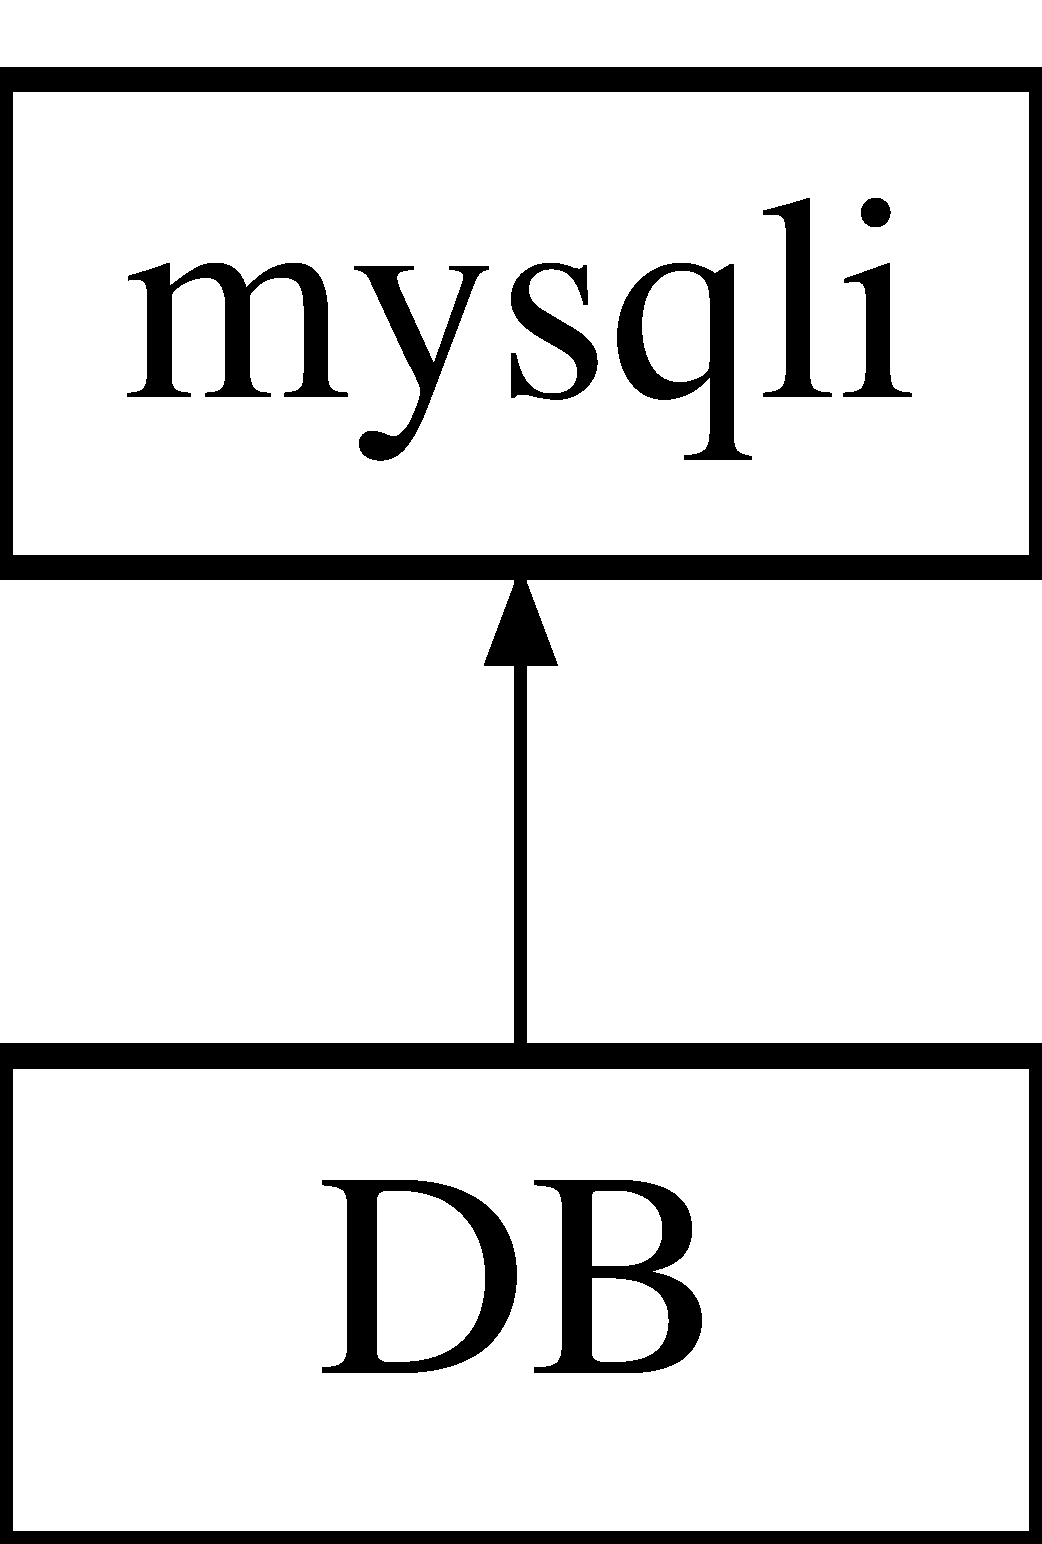
\includegraphics[height=2.000000cm]{class_d_b}
\end{center}
\end{figure}
\subsection*{Открытые члены}
\begin{DoxyCompactItemize}
\item 
\mbox{\Hypertarget{class_d_b_a03b8636c39cbba24d76581635186e5d2}\label{class_d_b_a03b8636c39cbba24d76581635186e5d2}} 
{\bfseries \+\_\+\+\_\+construct} (\$server\+Name, \$login, \$pass, \$db)
\item 
\hyperlink{class_d_b_ad1d77917cf531b111ab5ee86f1ca98c8}{query} (\$query, \$func=\char`\"{}\char`\"{}, \$error\+\_\+log=true)
\item 
\hyperlink{class_d_b_a59b7df33d9b7fcb2d9222c6f3823eab5}{q} (\$select, \$from, \$where=array())
\item 
\mbox{\Hypertarget{class_d_b_aa07dd114b2a3146de03aabf640688424}\label{class_d_b_aa07dd114b2a3146de03aabf640688424}} 
{\bfseries throw\+\_\+error} (\$funcname=\char`\"{}\char`\"{})
\item 
\mbox{\Hypertarget{class_d_b_a812cda4574715397b7ffd0be994adf10}\label{class_d_b_a812cda4574715397b7ffd0be994adf10}} 
{\bfseries escape} (\$string)
\end{DoxyCompactItemize}


\subsection{Подробное описание}
Перегружает некоторые функции стандартного класса mysqli. 

\subsection{Методы}
\mbox{\Hypertarget{class_d_b_a59b7df33d9b7fcb2d9222c6f3823eab5}\label{class_d_b_a59b7df33d9b7fcb2d9222c6f3823eab5}} 
\index{DB@{DB}!q@{q}}
\index{q@{q}!DB@{DB}}
\subsubsection{\texorpdfstring{q()}{q()}}
{\footnotesize\ttfamily q (\begin{DoxyParamCaption}\item[{}]{\$select,  }\item[{}]{\$from,  }\item[{}]{\$where = {\ttfamily array()} }\end{DoxyParamCaption})}

Функция делает запрос в базу данных с заданными параметрами. Запрещается использовать для выборки, в которой участвует более чем 1 таблица. Для этого необходимо использовать функцию \hyperlink{class_d_b_ad1d77917cf531b111ab5ee86f1ca98c8}{query()} 
\begin{DoxyParams}[1]{Аргументы}
array & {\em \$select} & Поля для выбора \\
\hline
string & {\em \$from} & Таблица, из которой идет выбор \\
\hline
array & {\em \$where} & Ассоциативный массив, где ключами являются поля, а значениями необходимые для отсеивания значения в соответствующих полях (могут быть массивы для сравнения на равенство). \\
\hline
\end{DoxyParams}
\mbox{\Hypertarget{class_d_b_ad1d77917cf531b111ab5ee86f1ca98c8}\label{class_d_b_ad1d77917cf531b111ab5ee86f1ca98c8}} 
\index{DB@{DB}!query@{query}}
\index{query@{query}!DB@{DB}}
\subsubsection{\texorpdfstring{query()}{query()}}
{\footnotesize\ttfamily query (\begin{DoxyParamCaption}\item[{}]{\$query,  }\item[{}]{\$func = {\ttfamily \char`\"{}\char`\"{}},  }\item[{}]{\$error\+\_\+log = {\ttfamily true} }\end{DoxyParamCaption})}


\begin{DoxyParams}[1]{Аргументы}
string & {\em \$query} & \\
\hline
bool & {\em \$error\+\_\+log} & \\
\hline
\end{DoxyParams}


Объявления и описания членов класса находятся в файле\+:\begin{DoxyCompactItemize}
\item 
model/classes/D\+B.\+php\end{DoxyCompactItemize}

\hypertarget{class_main}{}\section{Класс Main}
\label{class_main}\index{Main@{Main}}
\subsection*{Открытые члены}
\begin{DoxyCompactItemize}
\item 
\hyperlink{class_main_a0ff8cd567b3452dbfce15e57c16a3ce3}{use\+Controller} (\$c\+Name, \$settings=array())
\end{DoxyCompactItemize}


\subsection{Подробное описание}
Основной класс для управления системой. 

\subsection{Методы}
\mbox{\Hypertarget{class_main_a0ff8cd567b3452dbfce15e57c16a3ce3}\label{class_main_a0ff8cd567b3452dbfce15e57c16a3ce3}} 
\index{Main@{Main}!use\+Controller@{use\+Controller}}
\index{use\+Controller@{use\+Controller}!Main@{Main}}
\subsubsection{\texorpdfstring{use\+Controller()}{useController()}}
{\footnotesize\ttfamily use\+Controller (\begin{DoxyParamCaption}\item[{}]{\$c\+Name,  }\item[{}]{\$settings = {\ttfamily array()} }\end{DoxyParamCaption})}

Подключает контроллер с именем \$c\+Name. 
\begin{DoxyParams}[1]{Аргументы}
string & {\em \$c\+Name} & Название подключаемого контроллера. \\
\hline
array & {\em \$settings} & Параметры подключения контроллера. \\
\hline
\end{DoxyParams}
\begin{DoxyReturn}{Возвращает}
массив с результатом работы контроллера. Используется на странице подключения. Необходимо записать его в переменную и вывести результат в виде необходимого H\+T\+ML. 
\end{DoxyReturn}


Объявления и описания членов класса находятся в файле\+:\begin{DoxyCompactItemize}
\item 
model/classes/main.\+php\end{DoxyCompactItemize}

\hypertarget{class_user}{}\section{Класс User}
\label{class_user}\index{User@{User}}
\subsection*{Открытые члены}
\begin{DoxyCompactItemize}
\item 
\mbox{\Hypertarget{class_user_a12251d0c022e9e21c137a105ff683f13}\label{class_user_a12251d0c022e9e21c137a105ff683f13}} 
{\bfseries get\+Id} ()
\item 
\mbox{\Hypertarget{class_user_a8e1a01c7b21ec79c38e7d8e6b939ce27}\label{class_user_a8e1a01c7b21ec79c38e7d8e6b939ce27}} 
{\bfseries get\+Surname} ()
\item 
\mbox{\Hypertarget{class_user_a3d0963e68bb313b163a73f2803c64600}\label{class_user_a3d0963e68bb313b163a73f2803c64600}} 
{\bfseries get\+Name} ()
\item 
\mbox{\Hypertarget{class_user_a5e2103a61108304fcd718a517884ab5d}\label{class_user_a5e2103a61108304fcd718a517884ab5d}} 
{\bfseries get\+Third\+Name} ()
\item 
\mbox{\Hypertarget{class_user_a2b284f11184201a8ba8a92de57f93580}\label{class_user_a2b284f11184201a8ba8a92de57f93580}} 
{\bfseries get\+Full\+Name} ()
\item 
\mbox{\Hypertarget{class_user_a0cbfea8f34063f74136aa05476ba4107}\label{class_user_a0cbfea8f34063f74136aa05476ba4107}} 
{\bfseries get\+Surname\+Name} ()
\item 
\mbox{\Hypertarget{class_user_a4f44e7bc9de772c21b4304d11e87bf16}\label{class_user_a4f44e7bc9de772c21b4304d11e87bf16}} 
{\bfseries get\+Group} ()
\item 
\mbox{\Hypertarget{class_user_a934da130b87be052e8aa73da8fd4fc95}\label{class_user_a934da130b87be052e8aa73da8fd4fc95}} 
{\bfseries get\+Faculty} ()
\item 
\mbox{\Hypertarget{class_user_a23fac327059bf3fd0fe57555252d8cf2}\label{class_user_a23fac327059bf3fd0fe57555252d8cf2}} 
{\bfseries get\+Level} ()
\item 
\mbox{\Hypertarget{class_user_addca40e39caf569a9e7294803abb91cb}\label{class_user_addca40e39caf569a9e7294803abb91cb}} 
{\bfseries get\+Events\+Responsible\+Count} ()
\item 
\mbox{\Hypertarget{class_user_a91798b61f6df8d4c58338662c2fa3dd2}\label{class_user_a91798b61f6df8d4c58338662c2fa3dd2}} 
{\bfseries log\+In} (\$login, \$password)
\item 
\mbox{\Hypertarget{class_user_a5e2e988932fc4fdd67fbdad7f0c9c460}\label{class_user_a5e2e988932fc4fdd67fbdad7f0c9c460}} 
{\bfseries Count\+Events\+Responsible} ()
\item 
\mbox{\Hypertarget{class_user_a51abcf7a7d1795d49ccb73d7a8d9215e}\label{class_user_a51abcf7a7d1795d49ccb73d7a8d9215e}} 
{\bfseries get\+Num\+Post\+Notes} ()
\item 
\mbox{\Hypertarget{class_user_aa47914239932f3013b739ab0fde7ea08}\label{class_user_aa47914239932f3013b739ab0fde7ea08}} 
{\bfseries get\+Num\+Event\+Notes} ()
\item 
\mbox{\Hypertarget{class_user_af3d29bcb812373e739f5e5a464fc9121}\label{class_user_af3d29bcb812373e739f5e5a464fc9121}} 
{\bfseries get\+Num\+Task\+Notes} ()
\item 
\mbox{\Hypertarget{class_user_a1b72d4fb43da8989ee6a980d6e19c9e2}\label{class_user_a1b72d4fb43da8989ee6a980d6e19c9e2}} 
{\bfseries get\+Num\+Soc\+Notes} ()
\item 
\mbox{\Hypertarget{class_user_aafa6d6f1112024a9c435946704002246}\label{class_user_aafa6d6f1112024a9c435946704002246}} 
{\bfseries get\+Num\+Notes} ()
\end{DoxyCompactItemize}
\subsection*{Открытые статические члены}
\begin{DoxyCompactItemize}
\item 
\mbox{\Hypertarget{class_user_ad8bd251d2981e5ecefe88ba31d42a89c}\label{class_user_ad8bd251d2981e5ecefe88ba31d42a89c}} 
static {\bfseries Id} ()
\end{DoxyCompactItemize}


\subsection{Подробное описание}
Класс пользователя. 

Объявления и описания членов класса находятся в файле\+:\begin{DoxyCompactItemize}
\item 
model/classes/user.\+php\end{DoxyCompactItemize}

%--- End generated contents ---

% Index
\backmatter
\newpage
\phantomsection
\clearemptydoublepage
\addcontentsline{toc}{chapter}{Алфавитный указатель}
\printindex

\end{document}
